%! TEX root = main.tex

\graphicspath{{00_Images/05_chapter/}}

\chapter{Audio Filters and Equalization}
\label{ch:filters}

\section{Filter Classifications}
\label{sc:51}

Audio filters overlap considerably in their practical applications, yet they are systematically classified along several independent axes: the shape of their frequency response, whether they rely on active or passive components, the mathematical approximation used to approach the ideal response, and the order of the underlying transfer function.
Each of these dimensions captures a distinct design trade-off and together they provide the vocabulary needed to specify, analyze, and implement any filtering stage encountered in a professional audio chain.

\subsection{Frequency Response}
\label{sc:511}

The most immediate classification concerns the region of the spectrum that a filter passes or attenuates.
Four canonical responses are recognized in audio engineering, as illustrated in figure \ref{fig:filtersTF}.

\begin{figure}[!htb]
    \centering
    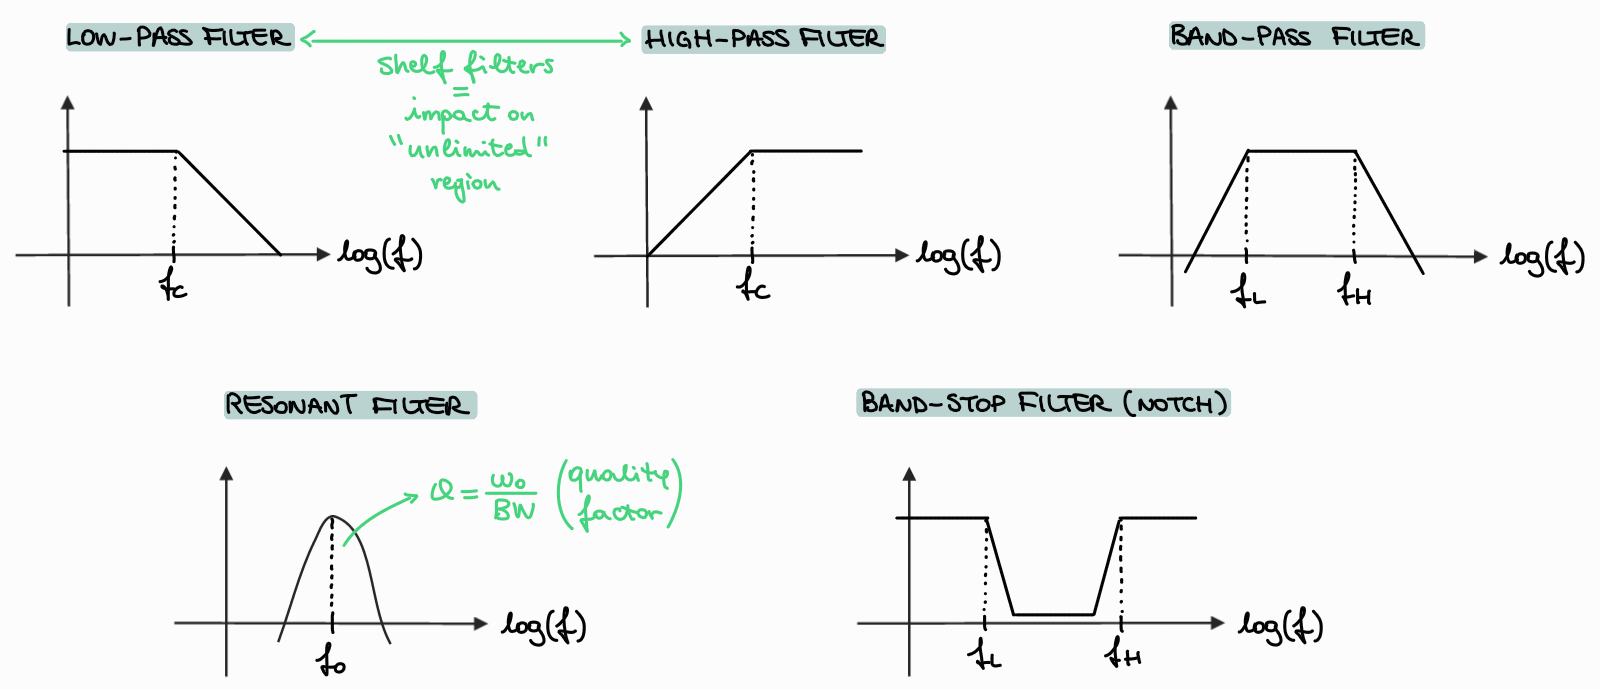
\includegraphics[width=0.90\textwidth]{Filters_TF.png}
    \caption{Transfer functions of the four canonical filter types: LPF, HPF, BPF, and BSF (notch)}
    \label{fig:filtersTF}
\end{figure}

\begin{itemize}
    \item A Low-Pass Filter (LPF), also called a high-cut filter in audio contexts, transmits all components below a cutoff frequency \( f_c \) and attenuates those above it.
    \item The complementary High-Pass Filter (HPF), or low-cut filter, passes frequencies above \( f_c \) while rejecting lower components.
    \item A Band-Pass Filter (BPF) selects a contiguous band of frequencies centered on \( f_0 \), attenuating both the low and high tails of the spectrum.
    \item The fourth type, the Band-Stop Filter (BSF), commonly called a notch filter, performs the inverse operation: it suppresses a narrow band centered on \( f_0 \) and passes everything else.
\end{itemize}

\paragraph{Resonant filters} A special and practically important subclass of BPF and BSF is the resonant filter, whose behavior is characterized not by its passband width alone but by the center frequency \( f_0 \) and the quality factor
\[
Q = \frac{f_0}{BW}
\]
where \( BW \) is the \( -\SI{3}{\decibel} \) bandwidth.
A high \( Q \) produces a narrow, selective peak or notch, while a low \( Q \) yields a broad, gentle shaping, a distinction central to parametric equalizer design.

\subsection{Active vs. Passive}
\label{sc:512}

A second classification distinguishes whether the filter uses only passive elements or incorporates active amplifying devices.

\paragraph{Passive filters} are constructed exclusively from resistors, capacitors, inductors, transformers, and gyrators.
They require no power supply and, since they cannot add energy to the signal, satisfy \( P_{out} < P_{in} \) at all times.
This property makes passive networks excellent choices for power-level crossover networks placed directly between a power amplifier and loudspeaker drivers, or for simple AC-coupling stages where galvanic isolation from a DC offset is needed.
The principal disadvantage is impedance coupling: the input impedance of a downstream stage loads the preceding filter, shifting its poles and zeros and modifying the intended frequency response in a way that depends on the connected circuitry.

\paragraph{Active filters} combine passive RC networks with operational amplifiers or transistor stages, and therefore require an external power supply with \( P_{out} \geq P_{in} \).
The key advantage is stage isolation: the OPAMP drives the output with very low impedance while presenting very high impedance at its input, so successive filter stages do not interact with one another.
A further benefit is the ability to realize complex-conjugate pole pairs, and hence second-order and higher-order filter responses with controlled damping, using only resistors and capacitors, entirely avoiding the bulky, lossy, and expensive inductors that equivalent passive designs would require.

\subsection{Approximation Type}
\label{sc:513}

The ideal ``brick-wall'' filter, which passes its band with perfectly flat gain and zero phase distortion while providing infinite attenuation outside it, is physically unrealizable because the corresponding impulse response would be non-causal.
Real filter design therefore consists of choosing a rational transfer function \( H(s) \) that approximates the desired ideal response according to a specific mathematical criterion; each criterion produces a distinct family of filters with characteristic trade-offs between passband flatness, transition-band steepness, and phase behavior.

\begin{figure}[!htb]
    \centering
    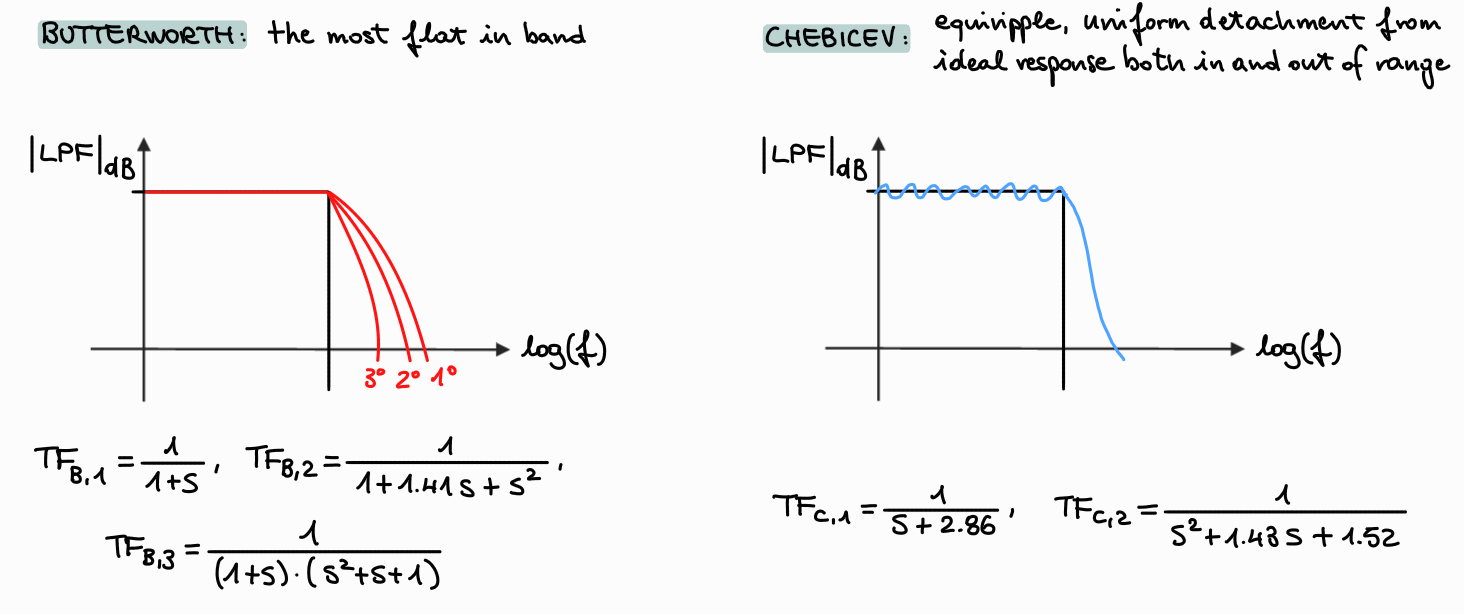
\includegraphics[width=0.90\textwidth]{Digital_LPF.png}
    \caption{Magnitude responses of Butterworth and Chebyshev approximations illustrating the trade-off between passband flatness and roll-off steepness}
    \label{fig:butterCheby}
\end{figure}

\begin{itemize}
    \item The Butterworth approximation maximises the flatness of the magnitude response in the passband: the first \( 2N-1 \) derivatives of \( |H(j\omega)|^2 \) are zero at \( \omega = 0 \), producing the so-called maximally flat response.
    The roll-off outside the passband is monotonically increasing with order but not as steep as other approximations of the same order.
    \item The Chebyshev approximation trades passband flatness for a steeper transition from passband to stopband.
    The magnitude response exhibits equiripple behavior in the passband, it oscillates between prescribed limits, which allows the roll-off to begin more abruptly.
    For a given filter order and transition bandwidth, the Chebyshev filter achieves greater attenuation in the stopband than the Butterworth at the cost of controlled passband ripple.
    \item The Bessel approximation optimizes for linear phase in the passband rather than magnitude flatness.
    A linear phase response implies constant group delay, meaning all frequency components in the passband are delayed by the same amount and therefore emerge undistorted in shape.
    This property is especially desirable in loudspeaker crossover networks, where preserving the temporal structure of transient signals matters for accurate stereo imaging and spatial reproduction.
\end{itemize}

\subsection{Filter Order}
\label{sc:514}

The order of a filter is defined as the highest power of \( s \) appearing in the denominator of its transfer function.
Physically, each order corresponds to one reactive element (capacitor or inductor) in the circuit and adds one pole to the transfer function.
The practical significance is that each additional order of filtering contributes a further asymptotic roll-off of \( -\SI{20}{\decibel\per decade} \) (equivalently \( -\SI{6}{\decibel} \) per octave) beyond the cutoff frequency, as shown in figure \ref{fig:filterOrder}.

\begin{figure}[!htb]
    \centering
    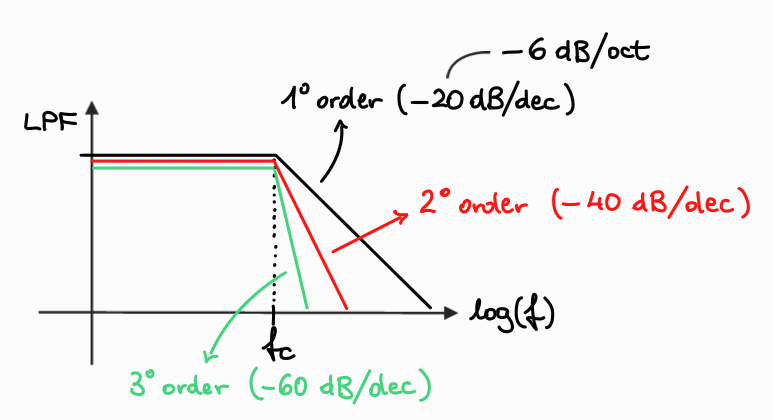
\includegraphics[width=0.50\textwidth]{Filter_Order_Illustration.png}
    \caption{Relationship between filter order and asymptotic roll-off slope: each additional order adds \( -\SI{20}{\decibel\per decade} \)}
    \label{fig:filterOrder}
\end{figure}

In the canonical Bode form, an \( N \)-th order transfer function is written as
\[
H(s) = K \cdot \frac{\prod_{i=1}^{N_z} (1 + s\tau_{z,i})}{\prod_{j=1}^{N_p} (1 + s\tau_{p,j})}
\]
where each real zero at \( f_{z,i} = 1/(2\pi\tau_{z,i}) \) increases the asymptotic slope by \( +\SI{20}{\decibel\per decade} \) and each real pole at \( f_{p,j} = 1/(2\pi\tau_{p,j}) \) decreases it by \( -\SI{20}{\decibel\per decade} \).
For a summary of the roll-off rates associated with the most common filter orders, refer to the table below.

\begin{center}
\begin{tabular}{|c|c|c|}
\hline
\textbf{Order} & \textbf{Attenuation per octave} & \textbf{Attenuation per decade} \\
\hline
1 & \( -\SI{6}{\decibel/\text{oct}} \) & \( -\SI{20}{\decibel/\text{dec}} \) \\
2 & \( -\SI{12}{\decibel/\text{oct}} \) & \( -\SI{40}{\decibel/\text{dec}} \) \\
3 & \( -\SI{18}{\decibel/\text{oct}} \) & \( -\SI{60}{\decibel/\text{dec}} \) \\
\hline
\end{tabular}
\end{center}

\section{Transfer Functions and Circuit Topologies}
\label{sc:52}

The generic second-order transfer function takes the form
\[
TF_2(s) = \frac{a_2 s^2 + a_1 s + a_0}{s^2 + b_1 s + b_0}
\]
which is known as a biquadratic function or biquad.
The denominator polynomial is common to all second-order filter types: it encodes the pole pair and determines the cutoff frequency and damping.
The numerator polynomial, by contrast, selects the filter type: setting \( a_2 = a_1 = 0 \) yields a low-pass response, setting \( a_1 = a_0 = 0 \) yields a high-pass response, and retaining only \( a_1 \neq 0 \) produces a band-pass response.
This elegant separation between pole placement (denominator) and response shaping (numerator) is what makes the biquad the fundamental building block of practical filter design, since any higher-order filter can be decomposed into a cascade of biquad sections.

\subsection{The Sallen–Key Topology}
\label{sc:521}

Among the many possible circuit realizations of the biquad, the Sallen–Key topology is notable for requiring only a single operational amplifier alongside a small number of passive RC components.
Unlike the standard inverting amplifier stage discussed in Chapter 2, which employs only negative feedback, the Sallen–Key filter exploits a simultaneous combination of negative feedback (which sets the gain) and positive feedback routed through the RC network (which controls the pole quality factor).

\begin{figure}[!htb]
    \centering
    \subfloat[Sallen–Key LPF schematic]{
        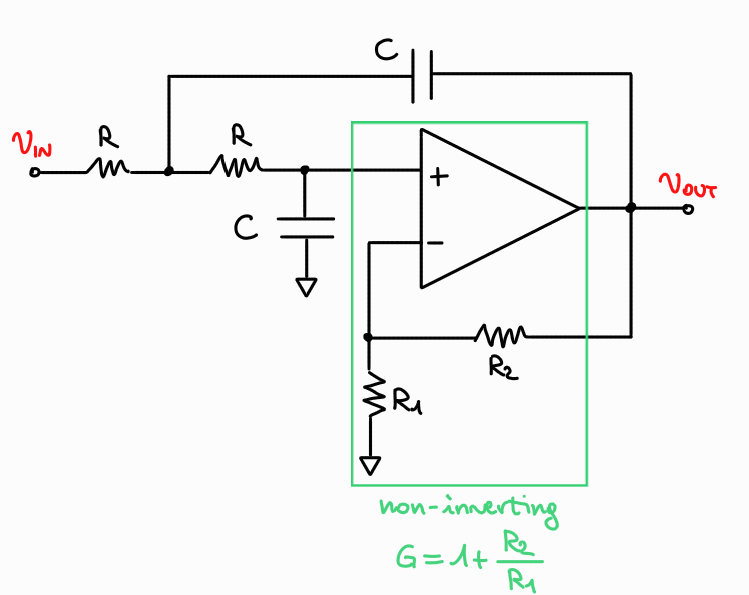
\includegraphics[width=0.45\textwidth]{Sallen_Key.png}
    }\hfill
    \subfloat[Equivalent block representation]{
        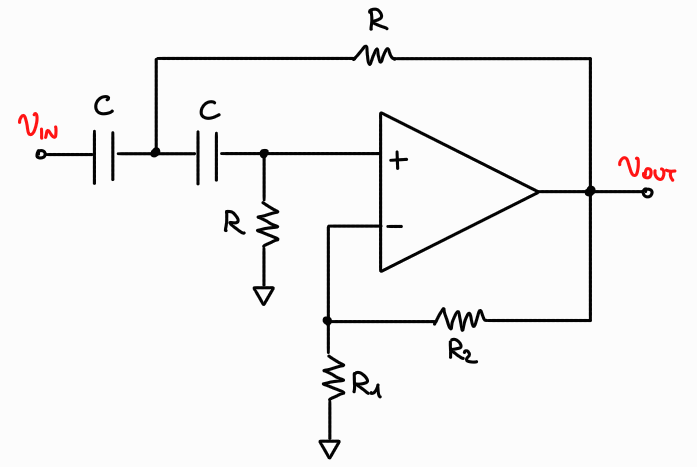
\includegraphics[width=0.45\textwidth]{Sallen_Key_dual.png}
    }
    \caption{Sallen–Key filter: single-amplifier second-order topology using simultaneous positive and negative feedback}
    \label{fig:sallenKey}
\end{figure}

The transfer function of the low-pass configuration is
\[
TF(s) = \frac{G}{s^2 \tau^2 + s(3 - G)\tau + 1}, \qquad \tau = RC
\]
where \( G \) is the DC gain set by the non-inverting amplifier stage.
The denominator shows clearly that the damping of the pole pair depends directly on \( (3 - G) \): as \( G \) approaches 3, the damping coefficient vanishes and the filter becomes marginally stable, with the poles reaching the imaginary axis.
For \( G > 3 \) the system becomes unstable.
The stability constraint therefore imposes \( G < 3 \), and in practice the gain is kept at 1 or 2 to provide adequate stability margin.
The general Sallen–Key transfer functions, written with explicit component values for both low-pass and high-pass configurations, are
\[
TF_{LP}(s) = \frac{G}{s^2 R_1 R_2 C_1 C_2 + s\left[(3-G)R_2 C_2 + R_1 C_1\right] + 1}
\]
and
\[
TF_{HP}(s) = \frac{G s^2 R_1 R_2 C_1 C_2}{s^2 R_1 R_2 C_1 C_2 + s\left[(3-G)R_1 C_1 + R_2 C_2\right] + 1}
\]
Both expressions deliver the second-order slope of \( -\SI{12}{\decibel/\text{oct}} \) in the stop-band and are widely encountered in professional mixing console input strips and crossover filter banks.

\begin{figure}[!htb]
    \centering
    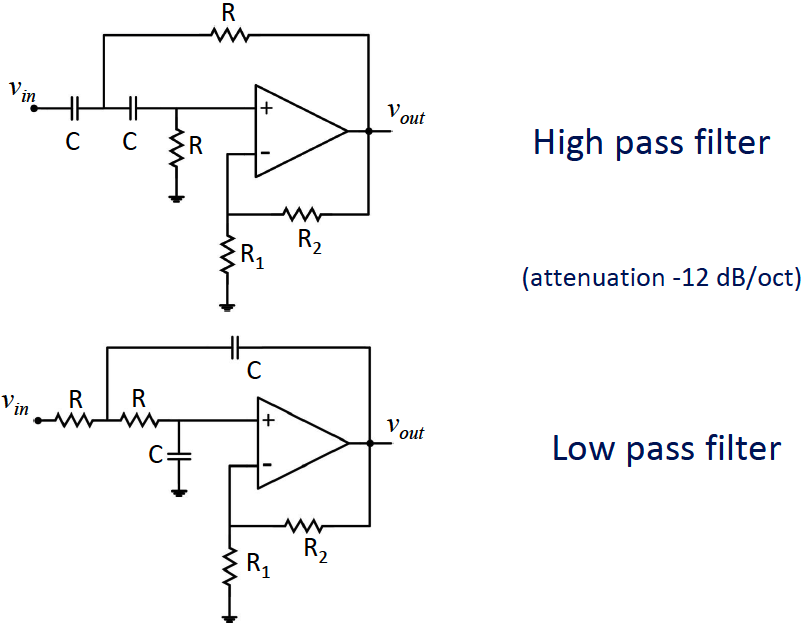
\includegraphics[width=0.60\textwidth]{Sallen_Key_Slides.png}
    \caption{Sallen–Key low-pass and high-pass circuit realizations used in tone control and crossover applications within professional consoles}
    \label{fig:sallenKeySlides}
\end{figure}

\section{Parametric Filters and Tone Control}
\label{sc:53}

\subsection{Parametric Filters}
\label{sc:531}

The inverting low-pass filter configuration of section \ref{sc:52} yields a gain \( G_{in,band} = R_2/R_1 \) and a time constant \( \tau = CR_2 \), so the cutoff frequency is \( f_p = 1/(2\pi R_2 C) \).
The gain–bandwidth product \( GBWP = G_{in,band} \cdot f_p \) is a constant for a given amplifier, which means that varying \( R_2 \) to shift \( f_p \) simultaneously alters \( G_{in,band} \), an undesirable coupling that would change the in-band level every time the cutoff is adjusted.

\begin{figure}[!htb]
    \centering
    \subfloat[Single-resistor parametric LPF]{
        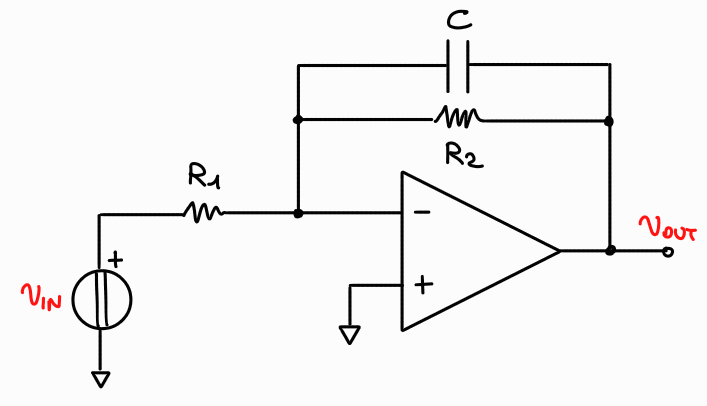
\includegraphics[width=0.45\textwidth]{Parametric_LPF.png}
    }\hfill
    \subfloat[Transfer function showing \( G_{in,band} \) dependence on \( R_2 \)]{
        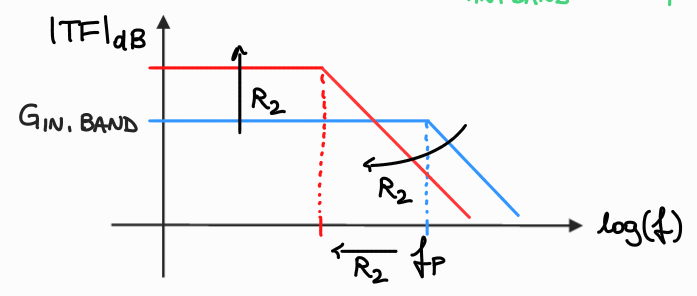
\includegraphics[width=0.45\textwidth]{Parametric_LPF_TF.png}
    }
    \caption{Basic parametric LPF: changing \( R_2 \) shifts the pole but also modifies the in-band gain, an undesirable coupling}
    \label{fig:parametricLPF}
\end{figure}

The solution is to replace both \( R_1 \) and \( R_2 \) with the two resistive sections of a dual (ganged) potentiometer \( P \), which enforces \( R_1 = R_2 = P \) at all settings.
Under the ideal OPAMP assumption \( v^+ = v^- = 0 \), the virtual-ground condition at the inverting input gives
\[
\frac{v_{in}}{P} + \frac{v_{out}}{P  ||  C} = 0
\quad \Rightarrow \quad
\frac{v_{out}}{v_{in}} = -\frac{1}{1 + sCP}
\]
The ratio \( R_2/R_1 = P/P = 1 \) is invariant, so \( G_{in,band} = 1 \) regardless of the potentiometer setting, while \( f_p = 1/(2\pi CP) \) is freely adjustable by rotating the knob, as confirmed by the family of curves in figure \ref{fig:parametricDualLPF}.

\begin{figure}[!htb]
    \centering
    \subfloat[Dual-potentiometer parametric LPF]{
        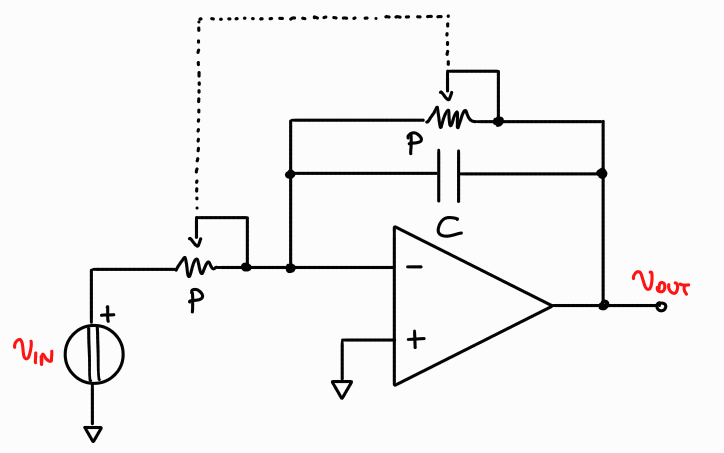
\includegraphics[width=0.45\textwidth]{Parametric_LPF_dual.png}
    }\hfill
    \subfloat[Transfer function: \( G_{in,band} \) is preserved for all values of \( P \)]{
        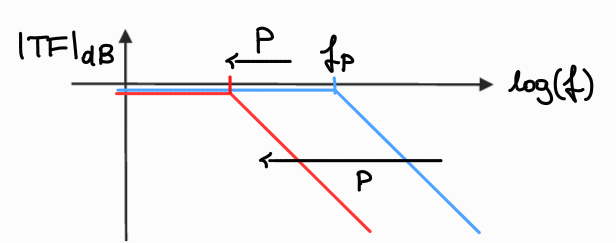
\includegraphics[width=0.45\textwidth]{Parametric_LPF_Dual_TF.png}
    }
    \caption{Dual-potentiometer parametric LPF: the ganged control shifts \( f_p \) without altering the in-band gain}
    \label{fig:parametricDualLPF}
\end{figure}

The same principle applies to the high-pass case: the capacitor is placed in series with the input branch and the potentiometer is moved to the feedback branch, yielding
\[
\frac{v_{out}}{v_{in}} = -\frac{sCP}{1 + sCP}
\]
which again preserves \( G_{in,band} = 1 \) for all values of \( P \), as shown in figure \ref{fig:parametricDualHPF}.

\begin{figure}[!htb]
    \centering
    \subfloat[Dual-potentiometer parametric HPF]{
        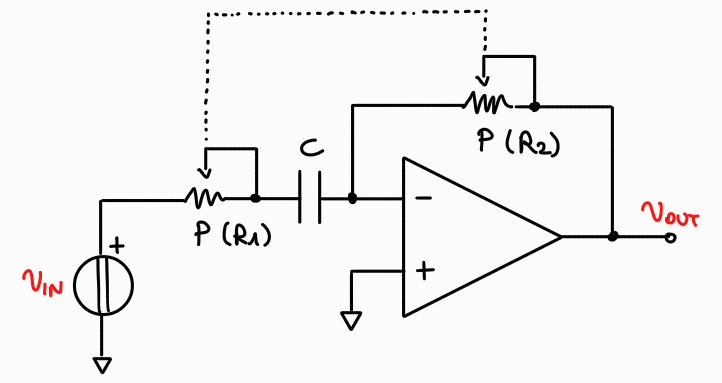
\includegraphics[width=0.45\textwidth]{Parametric_HPF_Dual.png}
    }\hfill
    \subfloat[Transfer function: \( G_{in,band} \) preserved across all values of \( P \)]{
        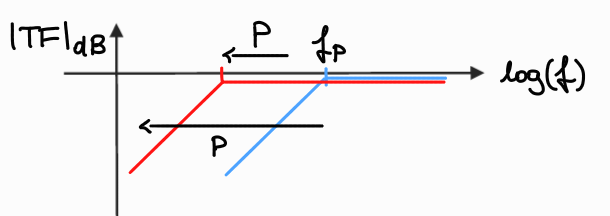
\includegraphics[width=0.45\textwidth]{Parametric_HPF__TF.png}
    }
    \caption{Dual-potentiometer parametric HPF: the same design principle as the LPF, applied symmetrically}
    \label{fig:parametricDualHPF}
\end{figure}

\subsection{Tone Control: Shelf Filters}
\label{sc:532}

Tone controls are a specialized class of filters intended to provide smooth, frequency dependent level adjustments over broad spectral regions rather than sharp cutoffs.
The characteristic response is a shelf: the gain transitions from one flat level to another across a transition band, creating a low-frequency or high-frequency plateau that can be boosted or cut relative to the mid-band reference.

\begin{figure}[!htb]
    \centering
    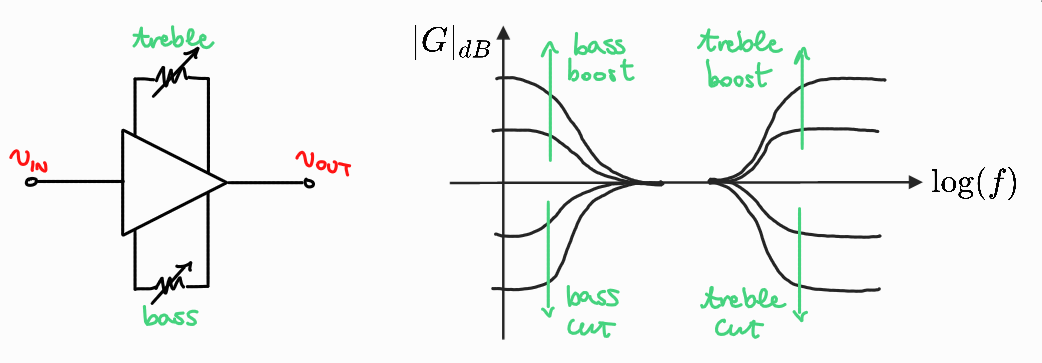
\includegraphics[width=0.90\textwidth]{Tone_Control_Filters_Gen.png}
    \caption{Frequency response of tone control shelf filters illustrating symmetrical boost and cut curves centered on the \( \SI{0}{\decibel} \) mid-point}
    \label{fig:toneControlGen}
\end{figure}

\paragraph{Bass-cut and bass-boost} Starting from an inverting OPAMP stage, a parallel RC network can be inserted either in the input impedance or in the feedback impedance to introduce a shelving zero and a shelving pole at different frequencies, thereby creating a slope between two flat regions.
Placing the RC network in the input branch gives a bass-cut transfer function with a zero at \( f_z = 1/(2\pi RC) \) and a pole at \( f_p = 1/\bigl(2\pi C(R  ||  R_1)\bigr) \), where \( f_p > f_z \):
\[
G_{BC}(s) = -\frac{R_1}{R + R_1} \cdot \frac{1 + s\tau_z}{1 + s\tau_p}, \qquad \tau_z = RC, \quad \tau_p = C(R  ||  R_1)
\]
Swapping the input and feedback impedances inverts the relationship and produces the complementary bass-boost:
\[
G_{BB}(s) = -\frac{R + R_1}{R_1} \cdot \frac{1 + s\tau_p}{1 + s\tau_z}
\]

\begin{figure}[!htb]
    \centering
    \subfloat[Bass-cut configuration: RC in the input branch]{
        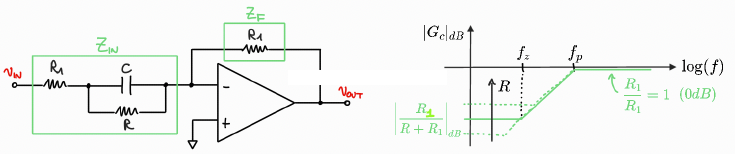
\includegraphics[width=0.70\textwidth]{Tone_Control_2.png}
    }\\
    \subfloat[Bass-boost configuration: RC in the feedback branch]{
        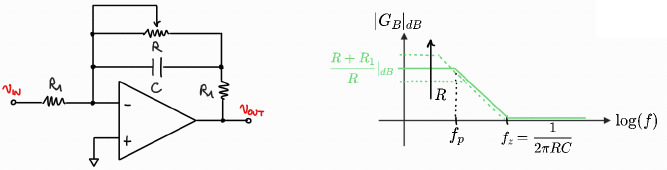
\includegraphics[width=0.70\textwidth]{Tone_Control_Bass_Boost.png}
    }
    \caption{Shelf filter circuits implementing bass cut (left) and bass boost (right) by swapping the input and feedback RC networks}
    \label{fig:bassShelf}
\end{figure}

The variable resistor \( R \) is the single control element: varying it shifts the gain of the shelf without altering the pole–zero spacing relative to the transition band.
In the complete bass-control stage the two complementary circuits are combined with a potentiometer so that rotating the knob from one extreme to the other sweeps continuously from maximum cut to maximum boost, passing through \( \SI{0}{\decibel} \) at the center position, as summarized below.
\[
\text{Bass Control:} \quad
\begin{cases}
\max \text{boost} = +K \text{dB} \\
\text{mid-point}   = \SI{0}{\decibel} \\
\max \text{cut}   = -K \text{dB}
\end{cases}
\qquad
f_z = \frac{1}{2\pi RC}
\]

\begin{figure}[!htb]
    \centering
    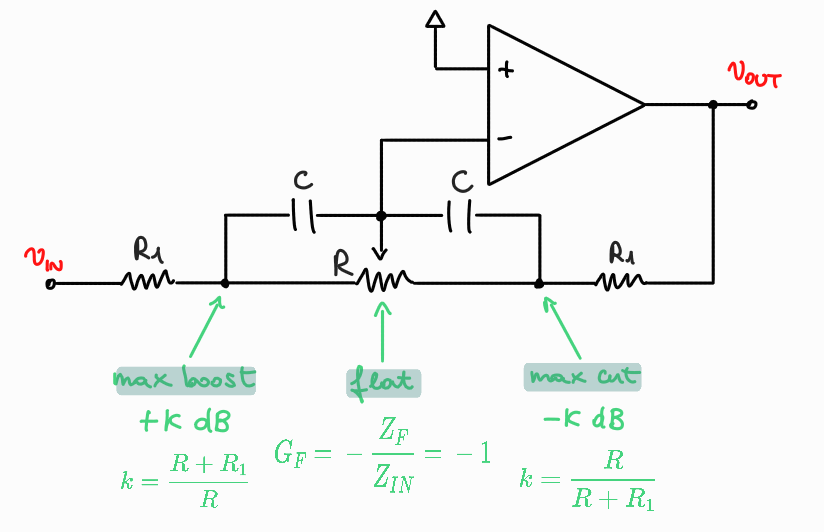
\includegraphics[width=0.75\textwidth]{Overall_Bass_Control.png}
    \caption{Complete bass-control stage combining boost and cut configurations through a single potentiometer}
    \label{fig:bassControl}
\end{figure}

An analogous derivation, applied to the high-frequency region, yields the treble-control stage with its own pair of complementary shelves, which are assembled in the same manner:
\[
\text{Treble Control:} \quad
\begin{cases}
\max \text{boost} = +K \text{dB} \\
\text{mid-point}   = \SI{0}{\decibel} \\
\max \text{cut}   = -K \text{dB} \\
\end{cases}
\qquad
f_p = \frac{1}{2\pi RC}
\]

\begin{figure}[!htb]
    \centering
    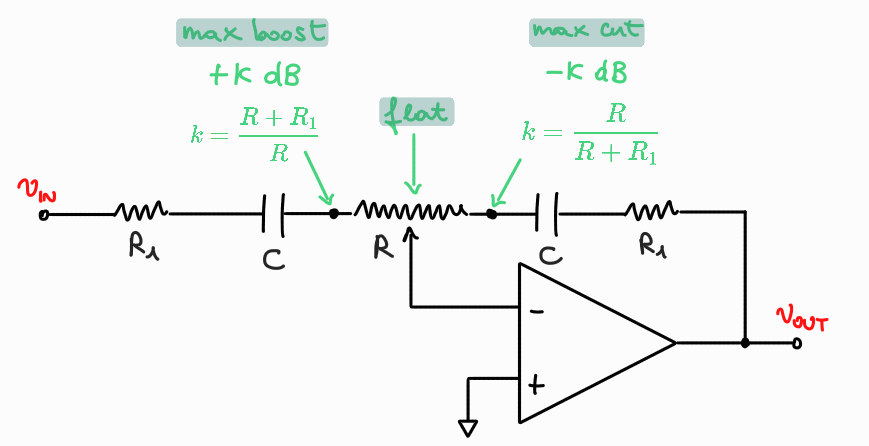
\includegraphics[width=0.65\textwidth]{Overall_Treble_Control.png}
    \caption{Complete treble-control stage, structurally analogous to the bass-control stage but acting on the high-frequency region}
    \label{fig:trebleControl}
\end{figure}

\paragraph{The Baxandall circuit} In professional audio equipment the bass and treble controls are almost universally combined into a single feedback network known as the Baxandall tone control, introduced by Peter Baxandall in 1952.
The key insight is that the OPAMP's virtual ground separates the bass-acting RC network from the treble-acting RC network, allowing each to operate independently within the same inverting stage without mutual interference.
The result is a smooth, symmetrical boost-and-cut characteristic with very low distortion, well-defined center frequency behavior, and interaction-free simultaneous control of both spectral extremes.
In high-fidelity integrated amplifiers such as the Luxman L-215, the Baxandall stage is inserted between the preamplifier output and the main amplifier input, ensuring that any tonal correction is applied at a low signal level before power amplification.

\begin{figure}[!htb]
    \centering
    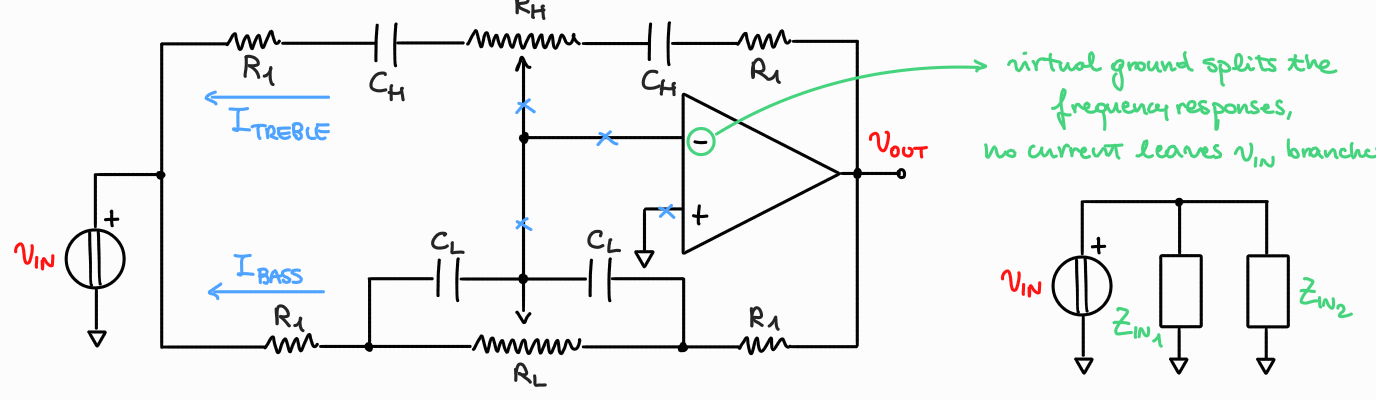
\includegraphics[width=0.90\textwidth]{Bakandall_Tone_Control.png}
    \caption{Baxandall tone control: bass and treble shelf networks combined within a single inverting OPAMP stage using virtual-ground frequency separation}
    \label{fig:baxandall}
\end{figure}


\section{Graphic vs. Parametric Equalizers}
\label{sc:54}

An equalizer is a filter bank in which multiple band-pass cells, each centered on a different frequency, are cascaded or summed so that the overall spectral response of a signal can be shaped with fine granularity.
The two principal families encountered in audio engineering, graphic and parametric, differ primarily in which parameters the operator is free to adjust.

\subsection{Parametric Equalizers}
\label{sc:541}

A parametric equalizer provides independent control over three parameters for each band: the center frequency \( f_0 \), the gain (boost or cut in \SI{}{\decibel}), and the quality factor \( Q \), which determines the bandwidth according to \( Q = f_0/BW \).
The core circuit element of each band is a tuneable band-pass filter, typically implemented as a state-variable or biquad section driven by an OPAMP.
The selectivity of the correction is governed by \( Q \): high \( Q \) values affect only a narrow spectral region, producing sharp surgical corrections, while low \( Q \) values produce broad, musically transparent shelving or bell-shaped adjustments.

\begin{figure}[!htb]
    \centering
    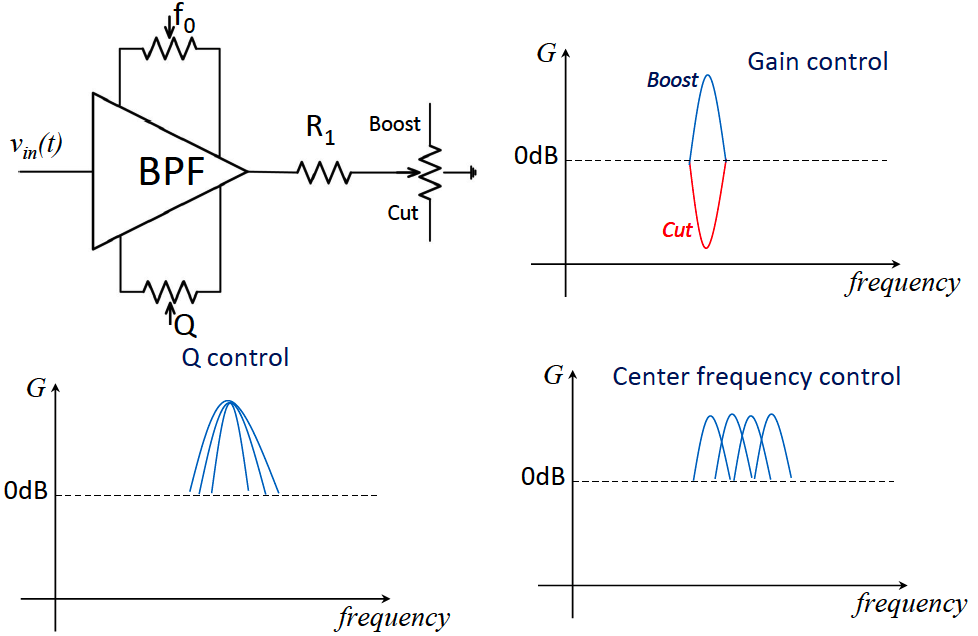
\includegraphics[width=0.75\textwidth]{Param_EQ.png}
    \caption{Parametric equalizer response: each band offers independent control of \( f_0 \), gain, and \( Q \), enabling precise spectral shaping}
    \label{fig:paramEQ}
\end{figure}

\subsection{Graphic Equalizers}
\label{sc:542}

A graphic equalizer fixes both the center frequencies \( f_0 \) of its bands and their quality factors \( Q \), leaving only the per-band gain as a user-adjustable parameter.
The center frequencies are spaced at standard octave or one-third-octave intervals, and each band is controlled by a vertical slider fader whose physical position gives an immediate visual representation of the overall frequency response, hence the name graphic.

\begin{figure}[!htb]
    \centering
    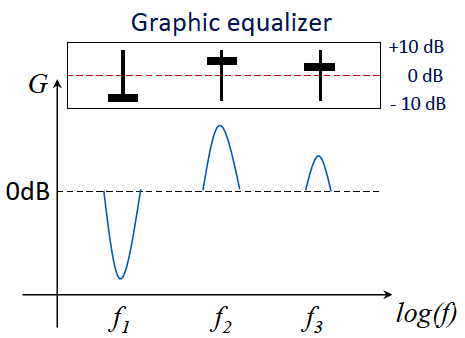
\includegraphics[width=0.40\textwidth]{Graphic_EQ.png}
    \caption{Graphic equalizer: sliders positioned at fixed frequencies \( f_i \) give the operator an immediate visual indication of the shaped frequency response}
    \label{fig:graphicEQ}
\end{figure}

\paragraph{Effect of the quality factor} The interaction between adjacent bands depends on their \( Q \) values.
High-\( Q \) cells produce narrow, selective peaks or dips with little influence on neighbouring bands, allowing independent per-band corrections.
Low-\( Q \) cells create broad, overlapping curves: boosting one band raises the gain of adjacent bands, so the effective correction deviates from the slider positions, as shown in figure \ref{fig:qFactor}.

\begin{figure}[!htb]
    \centering
    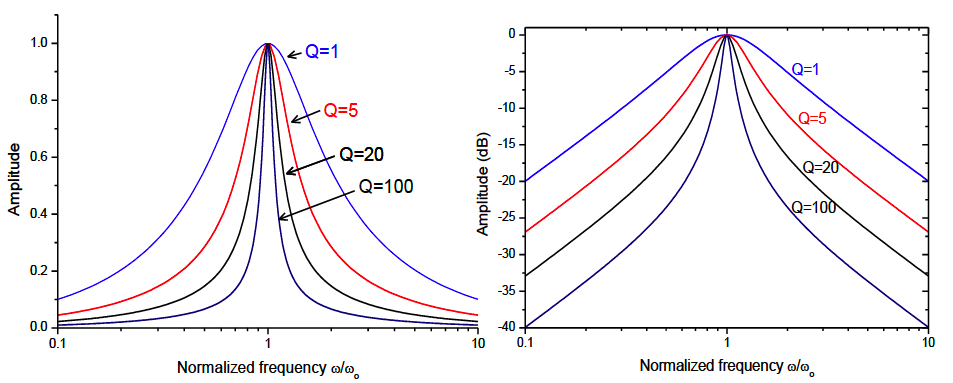
\includegraphics[width=0.90\textwidth]{Q_Factor.png}
    \caption{Influence of \( Q \) on the equalizer band response: higher \( Q \) produces a narrower, more selective peak or dip, while lower \( Q \) creates broader, overlapping corrections. Linear scale on the left, logarithmic scale on the right}
    \label{fig:qFactor}
\end{figure}

\subsection{Graphic Equalizer Circuit Implementation}
\label{sc:543}

The analogue circuit that underlies a graphic equalizer band can be understood by examining the dual-inverting-amplifier topology shown in figure \ref{fig:eqCircuit}.
The signal passes through two cascaded inverting OPAMP stages in series.
A passive band-pass filter \( RF_1 \), formed by a resonant RC network centered on the target frequency \( f_1 \), taps a filtered version of the signal and derives a frequency-selective current \( i_{f1} \).

\begin{figure}[!htb]
    \centering
    \subfloat[Base circuit with band-pass cell]{
        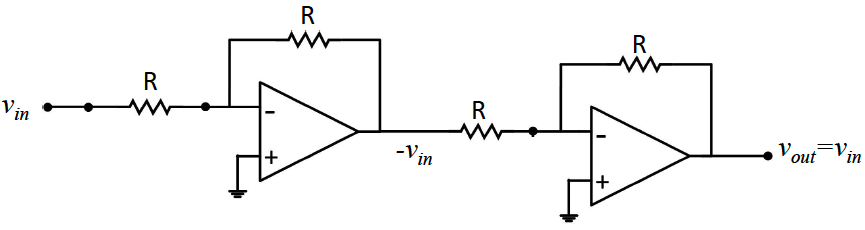
\includegraphics[width=0.45\textwidth]{EQ_circuit_1.png}
    }\hfill
    \subfloat[Flat response: potentiometer at center, \( i_{f1} \) contributes equally to both stages]{
        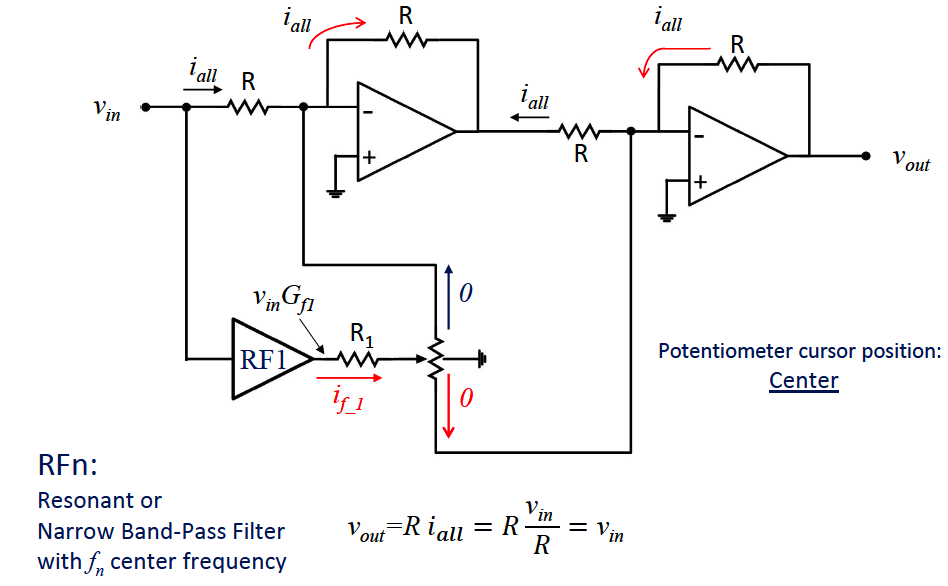
\includegraphics[width=0.45\textwidth]{EQ_Circuit_2.png}
    }
    \caption{Graphic equalizer analogue circuit: two cascaded inverting amplifiers with a band-pass cell extracting the frequency-selective current \( i_{f1} \)}
    \label{fig:eqCircuit}
\end{figure}

The position of the slider potentiometer determines into which amplifier the filtered current \( i_{f1} \) is injected, thereby selecting between boost and cut.

\begin{figure}[!htb]
    \centering
    \subfloat[Boost: potentiometer at top, \( i_{f1} \) injected into first stage]{
        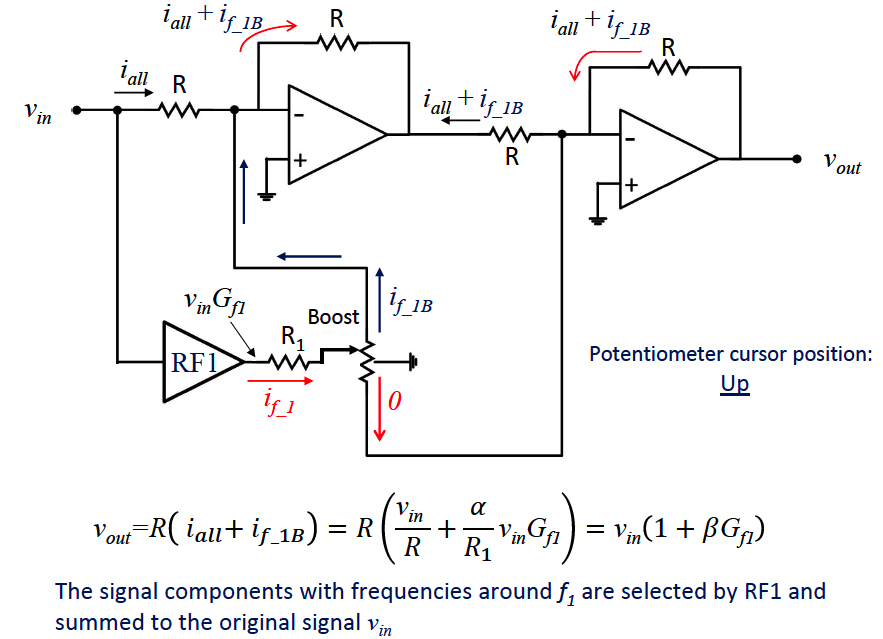
\includegraphics[width=0.45\textwidth]{EQ_circuit_3.png}
    }\hfill
    \subfloat[Cut: potentiometer at bottom, \( i_{f1} \) injected into second stage]{
        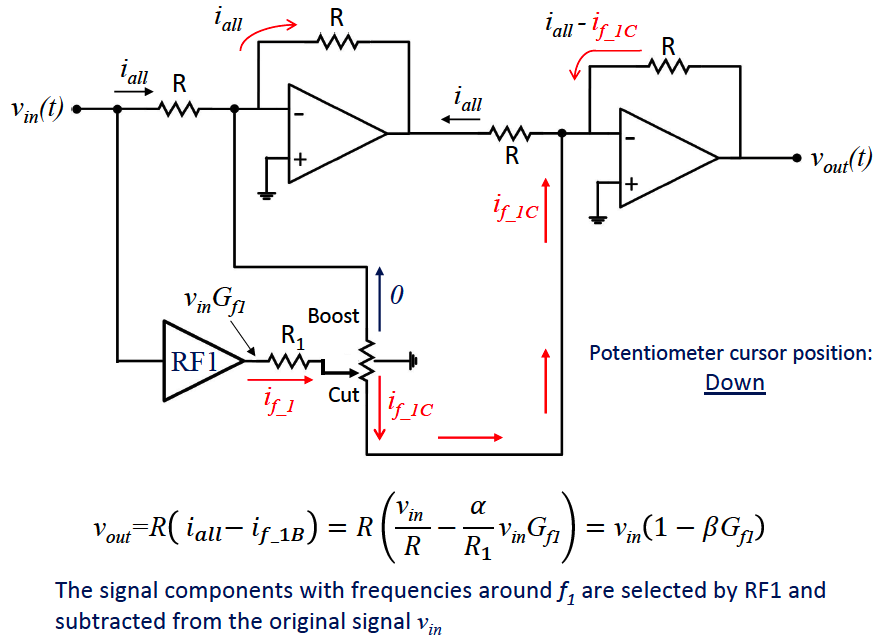
\includegraphics[width=0.45\textwidth]{EQ_circuit_4.png}
    }
    \caption{Boost mode (left) and cut mode (right) for the graphic equalizer band: the potentiometer position routes \( i_{f1} \) to the appropriate summation node}
    \label{fig:eqBoostCut}
\end{figure}

When the slider is moved to the top position, \( i_{f1} \) is injected into the virtual-ground node of the first inverting stage: since this current adds directly to the main signal current at that node, the contribution of \( f_1 \) is amplified and the band is boosted.
When the slider is moved to the bottom position, \( i_{f1} \) is injected into the virtual-ground node of the second inverting stage: at this point the main signal has already been inverted once by the first stage, so the filtered current opposes the (already-inverted) signal, producing a net reduction of the \( f_1 \) component, that is, a cut.
At the center position the current is split equally between the two nodes and the contributions cancel, yielding a flat response at \SI{0}{\decibel}.
The output of the graphic equalizer is taken after the second inversion, which restores the original polarity of the signal.
Because the band-pass filter \( RF_1 \) is passive, it operates as an approximate current divider, and the depth of the boost or cut scales linearly with the slider displacement from center.
Digital realizations of both graphic and parametric equalizers are now standard in DAW plug-ins and digital mixing consoles, where the same biquad transfer functions are implemented as IIR filters with computationally exact coefficient setting, enabling fully recallable and automation-friendly tone shaping.